% !TEX encoding = UTF-8 Unicode
\documentclass[11pt, a4paper]{article}
\usepackage[a4paper,left=2cm,right=2cm,top=3cm,bottom=3cm]{geometry}
\usepackage[utf8]{inputenc}
\PassOptionsToPackage{hyphens}{url}
\usepackage{fancyhdr}
\usepackage{mathrsfs,amsmath}
\usepackage{nccmath}
\usepackage{mathtools}
\usepackage{bm}
\usepackage{natbib}
\usepackage{caption}
\usepackage{float}
\usepackage{xcolor}
\usepackage{listings}
\usepackage{subfig}
\usepackage{placeins}
\usepackage{amsfonts,amssymb}
\usepackage{titlesec}
\usepackage{graphicx}
\usepackage{epstopdf}
\usepackage{float}
\usepackage{multirow}
%\usepackage{hyperref}
\usepackage{url}
\usepackage[nottoc,numbib]{tocbibind}
\usepackage{rotating}

\setcounter{secnumdepth}{4}
\setcounter{tocdepth}{2}
\lstset{language=MATLAB,
	        frame=single,
	        breaklines=true,
                basicstyle=\ttfamily,
                numbers=left,
                showstringspaces = false,
                keywordstyle=\color{blue}\ttfamily,
                stringstyle=\color{red}\ttfamily,
                commentstyle=\color{teal}\ttfamily,
                morecomment=[l][\color{magenta}]{\#},
                rulecolor=\color{black}
}

\pagestyle{fancy}
\fancyhf{}
\lhead{}
\chead{Final Year Project Interim Report 2022}
\rhead{}
\cfoot{\thepage}

\begin{document}\thispagestyle{empty}

\begin{titlepage}
% \newgeometry{top=25mm,bottom=25mm,left=38mm,right=32mm}
\setlength{\parindent}{0pt}
\setlength{\parskip}{0pt}
% \fontfamily{phv}\selectfont
{
    \Large
    \raggedright
    Imperial College London\\[17pt]
    Department of Electrical and Electronic Engineering\\[17pt]
    Final Year Project Interim Report 2022\\[17pt]
}

\rule{\columnwidth}{3pt}
\vfill
    \begin{center}
    \quad\\[1.1cm]
    
\includegraphics[width=7cm]{logo.png}\\[1cm]
    \end{center}\vfill
\setlength{\tabcolsep}{0pt}

\begin{tabular}{p{40mm}p{\dimexpr\columnwidth-40mm}}
    Project Title: & \textbf{Extraction of blood pressure from ECG and PPG signals} \\[12pt]
    Student: & \textbf{Arijit Bhattacharyya} \\[12pt]
    CID: & \textbf{01496199} \\[12pt]
    Course: & \textbf{MEng Electrical and Electronic Engineering} \\[12pt]
    Project Supervisor: & \textbf{Professor Esther Rodriguez Villegas} \\[12pt]
    Co Supervisor: & \textbf{Dr Zaibaa Patel} \\[12pt]
    Second Marker: & \textbf{Dr Christos Bouganis} \\[12pt]
\end{tabular}
\end{titlepage}

\newcommand{\HRule}{\rule{\linewidth}{0.5mm}}

\newpage
 \pagenumbering{roman}
%\section*{Abstract}


%\newpage
\tableofcontents
\newpage
\pagenumbering{arabic}
\newpage

\section{Introduction}
\subsection{Project Outline and deliverables}
This is the Interim Report for my Final Year Project, which is titled ”Extraction of blood pressure from ECG signals”. The report aims to present the initial background research and early implementation results. The report will contain the following sections as suggested in the project guide \cite{FYP2022}:\begin{itemize}
    \item \textbf{Project Specification}. This chapter will establish the expected deliverables of this project. The chapter will also describe the context of the underlying problem that the project will try to solve.
    \item \textbf{Background}. This chapter will first introduce the medical background, signal processing theories and machine learning principles needed to understand the project. A literature survey will be taken both to justify the proposed BP estimation method and for the justification of the use of wearable technology in future implementations.
    \item  \textbf{Implementation}. This chapter will describe what work has been done in regards to the chosen method for estimating blood pressure. In addition, a mathematical overview of the chosen implementation will be discussed in detail. Finally, the justification for using Python as the sole programming language for this project will be given.
    \item \textbf{Evaluation plan}. This chapter will detail how the project deliverables will be evaluated. In addition, the chapter will show the estimated timeline and possible extensions.
    \item \textbf{Ethical, Legal and Safety Considerations}. This chapter will
    look if there are any ethical legal or safety concerns both in regards to the project as is, but also briefly with potential extensions.
\end{itemize}


\subsection{Context}
Cardiovascular disease is one of the main causes of death around the world. High blood pressure (BP), which is also known as hypertension, is a common condition which can be a cause of cardiovascular disease \cite{Sharma2017}. According to the World Health Organization (WHO), the mortality rate due to hypertension is 9.4 million per year and it causes 55.3\%  of  total  deaths  in  cardiovascular patients \cite{Janjua2017}. If hypertension is detected early and prevented, this will greatly lower the number of deaths associated with cardiovascular diseases \cite{Janjua2017}. \\ \newline \noindent Recent developments in technology have made wearable sensors, such as Electrocardiogram (ECG) and Photoplethysmography (PPG) sensors significantly more popular in today's world. These sensors provide real-time 24 hour monitoring of the human bodily function. Hence there is great potential in using these sensors to diagnose medical conditions, such as hypertension, in real-time, thus helping to save lives \cite{Simjanoska20182}. Ambulatory BP monitoring is seen as a promising method for detecting early symptoms of hypertension \cite{Kario2021}. There is a lot of existing research to predict ambulatory BP using methods which are cuff-less, continuous and non-invasive \cite{Zaki2018}. Hence wearables are seen as a viable option for this. ECG and PPG sensors have been discovered to be a potential estimator of blood pressure that cause minimal harm to patients compared to existing cuff-based methods \cite{Malikeh2019} \cite{Bard2019}.\\ \newline \noindent The aim of this project is to implement and evaluate the different techniques that can be used to measure Ambulatory BP from ECG and PPG signals. The aims are to seek out implementations that have minimal computational complexity, whilst maintaining accuracy.


\newpage

\section{Background}
In this chapter, I will highlight all the necessary theory required to understand the basis of this project.
\subsection{Hypertension}
The heart can suffer from a variety of diseases and pathologies. Low blood pressure, or hypotension, has the potential to cause  a lack of oxygen flowing to the  brain  and  other  organs, causing shock \cite{Tanveer2018}, Whilst hypotension is a serious issue, hypertension has been identified by the World Health Organization (WHO) as the most significant risk factor for cardiovascular diseases \cite{Wang2018}. According to the 2017 American Heart Association guidelines for hypertension, the risk of developing stage two hypertension, $\ge 140$ mmHg systolic or $\ge 90$mmHg diastolic is almost 90\% \cite{Bard2019} (see Table 1 below). Over 20\% of adults have hypertension  and  its  complications  cause  a  major  number  of  dieases, including heart attacks, strokes and heart failure. If hypertension is not diagnosed and properly treated it can even cause death \cite{Janjua2017}. \\ \newline \noindent  Hypertension or high blood pressure (BP) is where blood continues to exert more and more pressure on the arterial walls. One particular disease linked to hypertension is hypertrophic cardiomyopathy, as indicated in Figure \ref{hypertension}, \begin{figure}[H]
    \centering
    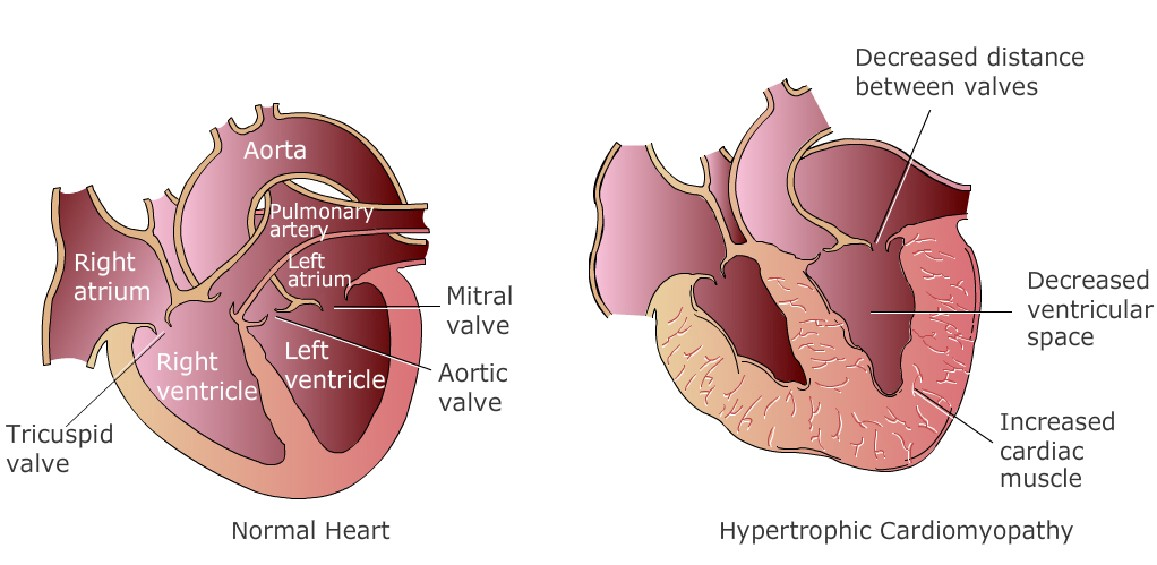
\includegraphics[width=12cm,height=12cm,keepaspectratio]{Figures/hypertension.jpeg}
    \caption{The effects of hypertension on the heart \cite{hypertrophic}}
    \label{hypertension}
\end{figure} \\ \newline \noindent Hence it is clear that hypertension is one of the largest motivating factors for this project.


\subsection{Blood Pressure measurements} 
Blood pressure (BP) is the force of the blood pushing against the arterial walls as the heart pumps blood. It is measured in millimeters of mercury (mmHg) \cite{Simjanoska20182}. BP  is  measured  in  terms  of  systolic  blood  pressure  (SBP)  and  diastolic  blood  pressure  (DBP). These values are the maximum and minimum pressure values of an arterial pressure tracing during a cardiac cycle respectively \cite{Simjanoska20181} \cite{Pradenas2020}.\\ \newline \noindent BP  has oscillations or pulses that mirror the oscillatory nature of the heart. The blood is propelled during systole, also known as heart contraction, and the blood is  rested during  diastole, known as heart  relaxation. \begin{figure}[H]
    \centering
    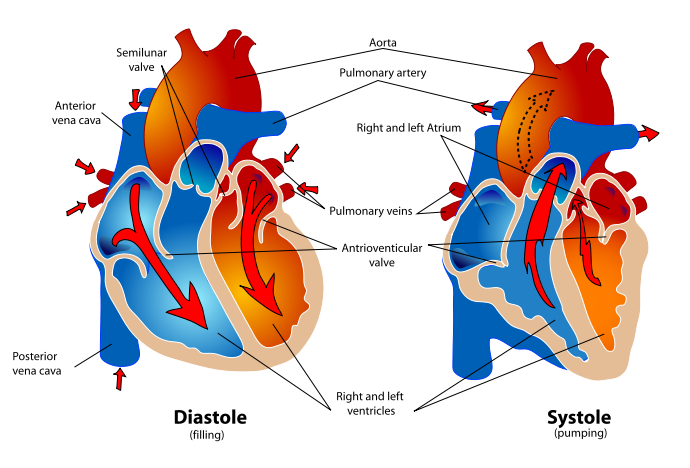
\includegraphics[width=12cm,height=12cm,keepaspectratio]{Figures/sbp_dbp.png}
    \caption{Visualisation for SBP and DBP \cite{SBP}}
    \label{hypertension}
\end{figure} \\ \newline \noindent There are two  conventional  methods  for  measuring  blood  pressure (BP). These are invasive   and   non-invasive methods. \\ \newline \noindent Firstly, a description on invasive methods. The most popular form of invasive  BP measurement is  catheterization \cite{Zaki2018}. Invasive BP measurements are continuous and the most accurate from heartbeat to heartbeat. As a result these measurements are recognised as the gold standard internationally \cite{Sharma2017} \cite{ElHajj2020}. However, this method is usually restricted to hospitals, as medical supervision is required \cite{Pradenas2020}. In addition, this method poses several health risks, including bleeding and infection. As a result, invasive measurements are only utilised for critically ill patients in intensive care units and for use during surgery \cite{Zaki2018}\cite{ElHajj2020}. \\ \newline \noindent Now a description on non-invasive methods. The gold standard for BP measurement is the use of a cuffed sphygmomanometer. Cuff-based methods provide BP measurements without any major side effects as opposed to BP measured invasively \cite{ElHajj2020}. However, patients will feel uncomfortable with long term monitoring due to the painful cuff inflation which interrupts the regular blood flow \cite{Tanveer2018}. In addition, these methods can only measure BP intermittently with intervals between measurements greater than at least two minutes. These devices are too cumbersome to wear during measurements. Also, it has been found that over three in ten home BP monitoring cuffs have produced inaccurate results \cite{Leung2016}. \\ \newline \noindent  As a result, the existing invasive and non-invasive BP measurement techniques are not feasible for an implementation involving continuous ambulatory BP monitoring \cite{ElHajj2020}. Hence, after having assessed the viability of all aforementioned methods, it is clear that it is difficult for these methods to be integrated with wearable technologies, which continue to gain popularity in commercial sectors and clinical practice \cite{Sharma2017}.
\begin{table}[H]
    \centering
\begin{tabular}{|c|cc|}
\hline
\multirow{2}{*}{\textbf{Blood pressure classification}} & \multicolumn{2}{c|}{\textbf{BP (mmHg)}} \\
 & \textbf{Systolic} & \textbf{Diastolic} \\ \hline
Hypotension & $\le$ 90 & And $\le$ 60 \\
Normal & $\lt$ 90-119 & And 60-79 \\
Prehypertension & 120-139 & Or 80-89 \\
Stage 1 hypertension & 140-159 & Or 90-99 \\
Stage 2 hypertension & $\ge$ 160 & Or $\ge$ 100 \\ 
Isolated Systolic hypertension & $\ge$ 140 & And $<$ 90\\
Hypertensive crisis & $\ge$ 180 & Or $\ge$ 110 \\ \hline
\end{tabular}
\label{bp_vals_table}
\caption{Categories of blood pressure in adults \cite{Wang2018} \cite{Simjanoska20181}}
\end{table}

\subsection{Ambulatory Blood Pressure (ABP)}
ABPM is when BP is measured as the patient moves around, and it allows patients to still live their normal daily lives \cite{Huang2021}. It has been classed as the gold standard for detecting and diagnosing hypertension and also assessing BP values over a 24 hour period \cite{Kario2021}. ABPM provides data on several important and unique parameters \cite{Kario2021}. This data can explain how changes in your BP may correlate with your daily activities and sleep patterns \cite{Huang2021}. Conventionally,  ABP is monitored by using a cuff attached to a portable device which is worn on the patient's waist \cite{Kario2021}. The 24-hour measurement duration is what makes this method a powerful tool to be used as a part of wearable technologies, which will be discussed later in Chapter 3. As mentioned previously, ECG and PPG signals have the potential to be used as an estimator for BP, and they will both be discussed now in more detail.

\subsection{Electrocardiogram (ECG) signals} ECG signals provide an overview of the electrical impulses occurring in the heart \cite{Simjanoska20181}. Electrical changes in the heart conduct through the body and are received at skin level. The record of these electrical fluctuations during the cardiac cycle is called the Electrocardiogram (ECG) \cite{Kumar2015}. The signals are recorded by measuring the electric potential difference by placing electrodes across the heart of an individual \cite{Tanveer2018} \cite{Simjanoska20181}. These electrodes are connected to the ECG machine with recordings from 12 different places on the body, which is known as the 12-lead ECG. The standard EKG leads are I, II, III, aVF, aVR, aVL, V1, V2, V3, V4, V5, V6. Leads I, II, III, aVR, aVL, aVF are classed as the limb leads and the others are precordial leads \cite{Tanveer2018}. \\ \newline \noindent The QRS complex of an ECG signal is detailed in Figure \ref{qrs}. This complex is first created through the generation of the electrical impulses from the heart.These signals then move along the electrical highway and as a result cause the ventricles to contract and pump oxygenated blood into the arteries. Physically, this whole describes the QRS complex \cite{Kumar2015}. \begin{figure}[H]
    \centering
    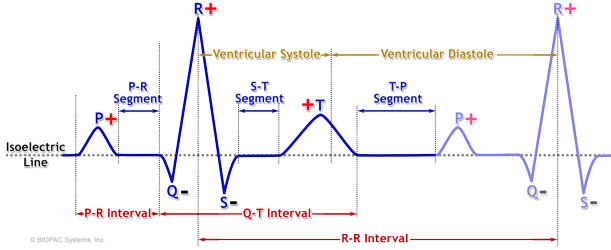
\includegraphics[width=12cm,height=12cm,keepaspectratio]{Figures/qrs.png}
    \caption{Structure of an ECG signal}
    \label{qrs}
\end{figure}
\subsection{Photoplethysmography (PPG) signals} 
Photoplethysmography (PPG) measures the blood volume changes per pulse. It is an optical and non-invasive technique that can determine a wide range of medical values, including an estimate for BP \cite{ElHajj2020}. Physically, the PPG signal is acquired by measuring the optical signal transmitted through or reflected  from  the  subject’s tissue \cite{Tanveer2018}. The PPG sensor consists of two components. The first component is an Light Emitting Diode (LED) to light up the surface of the skin. The second component is a photodetector, which is utilised for measuring the changes in light absorption over a period of time \cite{ElHajj2020} \cite{Kumar2015}. \begin{figure}[H]
    \centering
    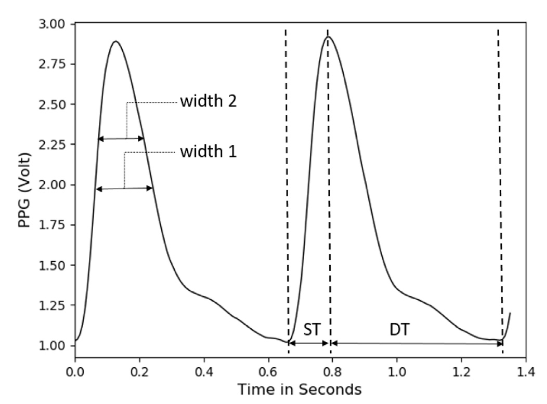
\includegraphics[width=12cm,height=12cm,keepaspectratio]{Figures/ppg.png}
    \caption{Structure of a PPG Signal \cite{ElHajj2020}}
    \label{ppg}
\end{figure} \noindent In Figure \ref{ppg}, the four features are the Systolic upstroke Time (ST), Diastolic Time (DT), width at $\frac{1}{2}$ amplitude (width 1) and width at $\frac{2}{3}$ amplitude (width 2) \cite{ElHajj2020}. PPG waveforms have a wide range of temporal features \cite{ElHajj2020}. These features have been utilised in several experimentations, creating  models  to  estimate blood pressure \cite{Pradenas2020}.

\subsection{Cuff-less methods for deriving BP} Cuff-less  methods have great potential in being used to estimate BP. This is because they provide continuous measurements, they cause minimal harm to the patients and they produce BP values over a long period of time  \cite{Liu2020}. There are three fundamental cuff-less methods which will now be discussed which can be used for deriving BP. These three methods rely on Pulse Transit Time (PTT), Pulse Arrival Time (PAT) and Pulse Wave Velocity (PWV) respectively \cite{Nye2015}. These will each now be discussed in more detail.

\subsubsection{Pulse Transit Time (PTT)} 
PTT is the time required for the arterial pressure wave to travel from the left ventricle to a distal arterial site. PTT holds an inverse relationship to blood pressure and as a result it is dependent on arterial compliance, arterial wall thickness, arterial radius, and blood density. PTT is conventionally found with the use of two PPG sensors \cite{Tanveer2018} \cite{Wang2018} \cite{ElHajj2020}, as indicated in Figure \ref{ptt}.
\begin{figure}[H]
    \centering
    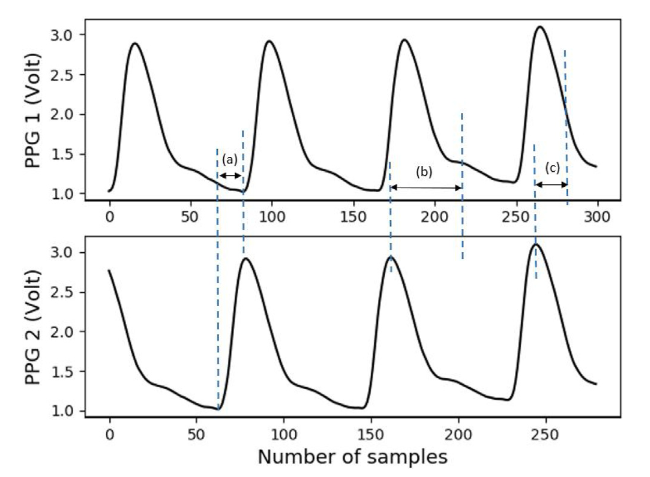
\includegraphics[width=12cm,height=12cm,keepaspectratio]{Figures/ptt.png}
    \caption{Pulse Transit Time (PTT) visualisation \cite{ElHajj2020}}
    \label{ptt}
\end{figure} \\ \newline \noindent It is important to note for Figure \ref{ptt} that the PTT can be measured at different points along the PPG waveforms. (a) represents a foot-to-foot time delay, (b) is a peak-to-dicrotic notch time delay and (c) is a peak to mid-point of the falling edge time delay \cite{ElHajj2020}. As a proof of concept, increasing BP leads to an increase in the tension along the arterial wall tension, which therefore reduces the PTT. Hence, the opposite also applies \cite{Kumar2015}.

\subsubsection{Pulse Arrival Time (PAT)} 
The PAT is the difference in time between the R-peak of the ECG signal and the systolic peak of the PPG signal when measured during the same cardiac cycle, as indicated in Figure \ref{pat} \cite{ElHajj2020} \cite{Malikeh2019}. Physically, PAT is the interval in time between the activation of electrical impulses at the heart and the arrival of the pulse wave at a location on the body, such as the finger \cite{Jeong2021}. PAT is measured using two sensors, an ECG and a PPG sensor \cite{ElHajj2020}. \begin{figure}[H]
    \centering
    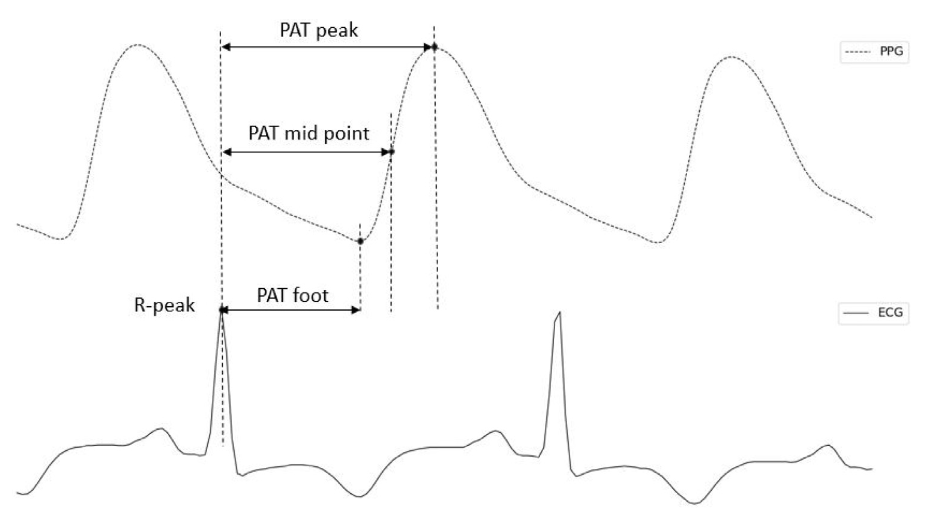
\includegraphics[width=12cm,height=12cm,keepaspectratio]{Figures/pat.png}
    \caption{Pulse Arrival Time (PAT) visualisation \cite{ElHajj2020}}
    \label{pat}
\end{figure} \\ \newline \noindent The Pre-ejection Period (PEP) delay can also be briefly discussed. PEP is the time needed to convert the electrical signal into a mechanical pumping force and isovolumetric contraction to open the aortic valves, \begin{align}
    PAT = PTT + PEP
\end{align}

\subsubsection{Pulse Wave Velocity (PWV)}
The PWV calculates the velocity of the pulse wave using two PPG sensors located on the same arterial branch at a known distance apart \cite{Pradenas2020} \cite{ElHajj2020}. The relation between PTT and PWV can be expressed as \begin{align}
    PWV = \frac{d}{PTT}
\end{align} where $d$ is the arterial distance travelled by the pressure wave. PWV is related to the Young's modulus of the vessel wall by the Moens-Kortweg equation, \begin{align}
    PWV = \sqrt{\frac{Eh}{\rho d}}
\end{align} where \\ \newline \noindent \begin{flushleft*}
    PWV &= Velocity of the pulse wave (m/s)\\
    E &= \text{ Young's modulus of vessel wall (Pa)}\\
    h &= \text{ vessel thickness (m)}\\
    \rho &= \text{ blood density (kg/$m^3$)}\\
    d &= \text{ arterial diameter (m)}\\
\end{flushleft*}\\ \newline \noindent The Young's modulus of the vessel wall is then related to the arterial pressure by the Bramwell-Hills equation, \begin{align}
    E = E_0 e^{\lambda P}
\end{align}where $E_0$ and $\lambda$ depend  on  the  thoracic  and abdominal aortas and P is the vessel blood pressure (mmHg) \cite{Janjua2017} \cite{Tanveer2018} \cite{Yang2020}. \\ \newline \noindent By solving Equations (2) and (3), we have the final equation for estimated blood pressure as, \begin{align}
    P = \frac{1}{\lambda} \ln{(2 r \rho \frac{\Delta X^2}{E_0 h})} - \frac{2}{\lambda} \ln{(PTT)}
\end{align} \\ \newline \noindent where \\ \newline \noindent \begin{flushleft*}
    r &= $\frac{d}{2}$ = \text{ arterial radius}\\
    \Delta X &= \text{ distance from heart to vessel}\\
\end{flushleft*}

\subsubsection{Limitations}
The blood pressure (BP) can be derived through mathematical models as soon as estimates have been calculated for PTT, PAT and PWV. Although these models are common approaches for BP monitoring in an environment that is non-invasive and cuff-less, there are many challenges to these implementations. As a result, none of these techniques by themselves have been established as a reliable indicator for the estimation of BP. \\ \newline \noindent Firstly, all three of the aforementioned methods require two separate measurements from two synchronised sensor devices. This can be a very inconvenient process for patients who are uncomfortable with this method \cite{Jeong2021}. \\ \newline \noindent In addition, there is a very likely possibility that these sensor devices will have different real-time sampling rates. Their operability depends on rather complicated arterial wave propagation models \cite{ElHajj2020}. \\ \newline \noindent In order to be able to continuously measure BP, constant calibration of the methods is required. This is due to individual patients having different physiological parameters \cite{Jeong2021}. \\ \newline \noindent Finally, even with per-person calibration, these models can only provide BP estimation for a short period of time. As a result, this makes the models unreliable for the estimation of BP with every heartbeat \cite{ElHajj2020}. \\ \newline \noindent To conclude this chapter, there is a lot of potential in the use of the three above parameters in the estimation of Ambulatory BP. However, there are still overarching limitations which currently hinder the progress of these parameters. As it will be discussed in Chapter 4, it will be indicated that these parameters still play a role in the estimation process but in methods which are more data driven.
\newpage 
\section{Overview on Cuff-Less BP device options} Wearable technology provides an opportunity for real-time monitoring of human vital signs, thus enabling the possibility for preventive, timely notification and real-time diagnosis. Unlike commonly-used BP sensors, which demand a specific measurement procedure, modern wearable bio-sensors monitor vital signals online and all day long, presenting no additional burden other than wearing the device.  A wide range of wearable devices achieve very positive results, even those wearables which are cheaper in price \cite{Simjanoska20182}. Some of the systems developed for the purpose of non-invasive BP monitoring will be discussed in more detail now. In addition, they will be critically analysed against two other viable alternatives. \\ \newline \noindent The motivation behind this project is to replace the current cuff-based BP devices. Cuff-based devices often require the supervision of an expert to work correctly and do not provide continuous measurements for BP. In addition they can cause irritation and inconvenience for patients due to cuff inflation and deflation. As a result, current clinical cuff-based BP devices are not suitable for providing continuous BP monitoring which could play a significant role in the early detection of diseases which affect the heart \cite{ElHajj2020}.

\subsection{Smart Watches}
Smart watches are becoming an increasingly popular form of wearable technology \cite{Bard2019}. Most of the existing smart watch produces currently measure BP through Pulse Transit Time (PTT) from a pulse wave measurement at the wrist. The Heartisans BP smartwatch uses ECG and PPG signals to measure PTT and estimate BP. The watch requires a motionless 20 second scan with the device held at heart level for measurements and provides systolic and diastolic BP readings. Calibration with a validated cuff-type BP device is required prior to standalone use. Despite its availability on the market, the Heartisans Watch has not undergone a formal validation study \cite{Bard2019}. \\ \newline \noindent Another wearable method  is  through  arterial  tonometry. The BPro device, developed by the London company HealthSTATS Technologies, is one such device. \begin{figure}[H]
    \centering
    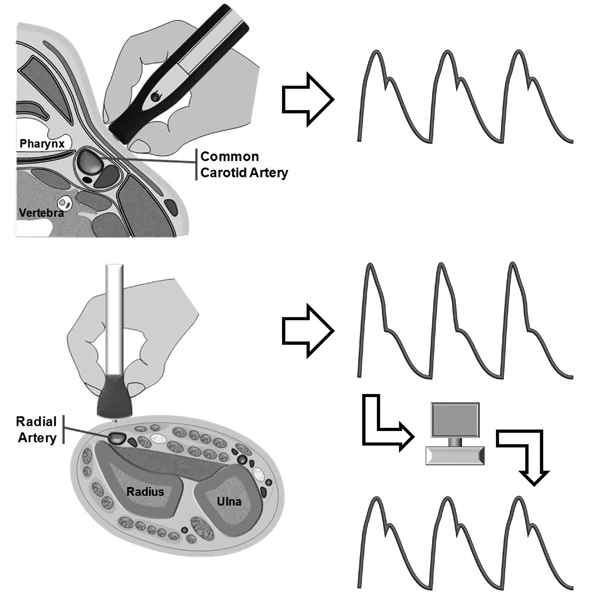
\includegraphics[width=6cm,height=6cm,keepaspectratio]{Figures/arterial.png}
    \caption{Arterial Tonometry}
    \label{tonometry}
\end{figure} \noindent Figure \ref{tonometry} shows two different methods for using arterial tonometry to measure blood pressure. The first image shows that the recording is taking at the carotid artery level in order to estimate the central blood pressure waveform. In the second image, the recording is taken at the radial artery level to estimate the arterial pulse wave. The central waveform is then reconstructed from this pulse wave using software. \\ \newline \noindent The BPro allows for continuous  24 hour  waveform  analysis  of  BP. Calibration to the brachial artery BP is required using a validated upper arm cuff device prior to use. The BPro has been validated in a non-ambulatory study following the Association for the Advancement of Medical Instrumentation (AAMI) standards and the European Society of Hypertension (ESH) protocol.

\subsection{Smartphone Applications}
Smartphones offer a great potential to expand the continuous recording of BP if their sensors can be correctly utilised \cite{Bard2019}. A formal validation study on one particular iOS application, the Instant Blood Pressure app, revealed poor accuracy of BP measurements. Mean absolute differences of 12.4 mmHg for systolic BP and 10.1 mmHg for diastolic BP were found between the Instant Blood Pressure application and a reference device. This resulted in approximately four out of five hypertensive individuals being falsely classified as normotensive  \cite{Bard2019}. The My BP Lab application measures BP through measurements of Pulse Transit Time (PTT). However, there is currently a lack of experimental data to justify it's dominance in the market.

\subsection{Medical Tricorders}
A medical tricorder is a handheld portable device used by consumers to self-diagnose medical conditions and take basic vital signs measurements. The   BodiMetrics   Performance   Monitor uses ECG and PPG signal data to estimate BP through PTT. The Bodimetrics tricorder obtains measurements with a 20 second scan of the user’s fingertip at heart level but only provides systolic BP data. This tricorder has a large spread in absolute bias against an automated sphygmomanometer, hence it is unlikely to meet formal accuracy and precision standards \cite{Bard2019}. \\ \newline \noindent The FreeScan Personal Cardiovascular Monitor, which is developed by the Taiwanese company Maisense Inc., also estimates BP from PTT. However the device uses a force sensor to capture the systolic arterial waveform rather than PPG. This requires the user to physically apply the force sensor directly to the radial artery for around 10 seconds for measurements. The Freescan device has been verified according to the AAMI protocol \cite{Bard2019}. \\ \newline \noindent The SOMNOtouch NIBP is a non-traditional medical tricorder that utilizes PTT data collected in a similar fashion to the Bodimetrics Performance Monitor. The device has met the ESH standards, however it begins to lose accuracy for higher SBP and DBP values \cite{Bard2019}.

\subsection{Conclusion}
After having discussed three viable devices for cuff-less measurements of BP, it has been finalised that smart watches are the most viable option. Whilst existing smart watch devices do suffer from inaccuracies in BP estimation due to motion, it is clear that they produce the most acceptable results in line with the AAMI and ESH standards. This chapter can be seen as a forward looking overview of how the estimation methods discussed in this report can be used to benefit future products. With regards to this project, this chapter can be treated as a supplementary overview.
\newpage
\section{Non-Invasive Cuff-Less Machine Learning methods for estimating BP}
Due to advancements in technology related to machine learning, there has been a lot of research into neural networks algorithms that can offer continuous BP measurements that are non-invasive and also cuff-less \cite{Pradenas2020}. These ML models have been seen to be based on the parameters mentioned in Chapter 2.6 (namely Pulse Transit Time, Pulse Arrival Time and Pulse Wave Velocity). However, in this case BP estimation is motivated by how much data is available to the algorithm \cite{ElHajj2020}. \\ \newline \noindent Artificial neural networks (ANNs) are a machine learning method that can be used to estimate blood pressure \cite{Pradenas2020}. ANNs are based on the neural networks found in the human body and aim to replicate their behaviour \cite{Yang2020}. The structure of ANN consists of multiplie individual units called neurons. Each neuron has five critical components. These are inputs, weights, transfer function, activation function and bias \cite{deeplearning}.  \begin{figure}[H]
    \centering
    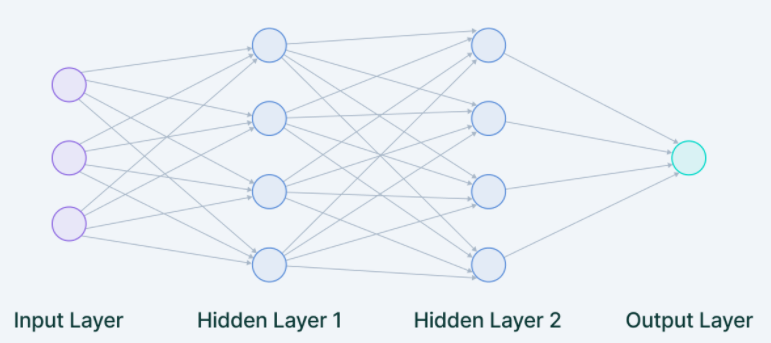
\includegraphics[width=10cm,height=10cm,keepaspectratio]{Figures/ann.png}
    \caption{Structure of a multi-layer ANN}
    \label{ann}
\end{figure}

\subsection{Convolutional Neural Networks (CNNs)}
Convolutional Neural Networks (CNNs) are a class of feed-forward artificial neural architecture. The basic pipeline of common CNNs consists of an image as input and a stack of convolutional layers that extract a feature representation from the input image. The final shape of the image representation is conditioned on the type of problem/task that the architecture is facing. For instance, the output of the last layer in a classification problem is a probability vector. Each dimension of the probability vector represents how likely is that the input image belongs to a specific class. However, the architecture design is customisable, and therefore it is possible to code a network that outputs a single value for regression problems, or for example that generates a new image map for semantic segmentation. \\ \newline \noindent One popular CNN architecture is the Residual Neural Network (ResNet) architecture, as depicted in Figure \ref{resnet}. ResNet is built by micro-architecture modules, called residual blocks. Those blocks introduced skip connections, which allowed to train huge architectures (152 layers) while still maintaining a lower complexity than other popular CNN architectures, such as VGGNet \cite{deeplearning}. Thus, residual connections allowed authors to design deeper architectures since the gradient could backpropagate easier through the skip connections.\begin{figure}[H]
    \centering
    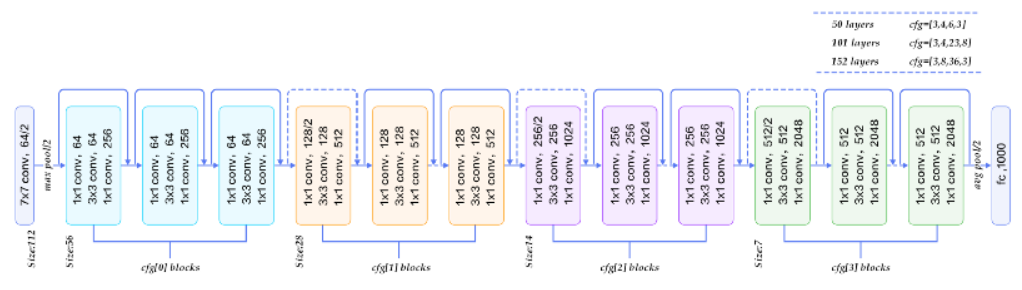
\includegraphics[width=15cm,height=15cm,keepaspectratio]{Figures/resnet.png}
    \caption{Architecture of the ResNet CNN with skip connections}
    \label{resnet}
\end{figure}


\subsection{Recurrent Neural Networks}
A Recurrent Neural Network (RNN) is a specific type of architecture that is widely used to deal with sequential information \cite{rnns}. \\ \newline \noindent RNNs are called recurrent since they apply the same operation to each of the input sequences, with the output of an individual element being dependent on the previous one. Theoretically, RNNs establish a connection between the actual input and ALL the previous ones \cite{rnns}. Although this is assumed, in the practice, RNNs have proven to only remember a limited number of inputs. In other words, RNNs have a memory that allows them to remember previous elements and use their information to deal with the current input \cite{deeplearning}. \\ \newline \noindent RNNs can be split into multiple types depending on their applications. For instance, if we want to predict one word given only the previous one, the topology of our network is a One to One. Another example is image captioning, where we can design a One to Many architecture to obtain a description from a single input image \cite{rnns}. The following diagram shows the different types of problems we can face: \begin{figure}[H]
    \centering
    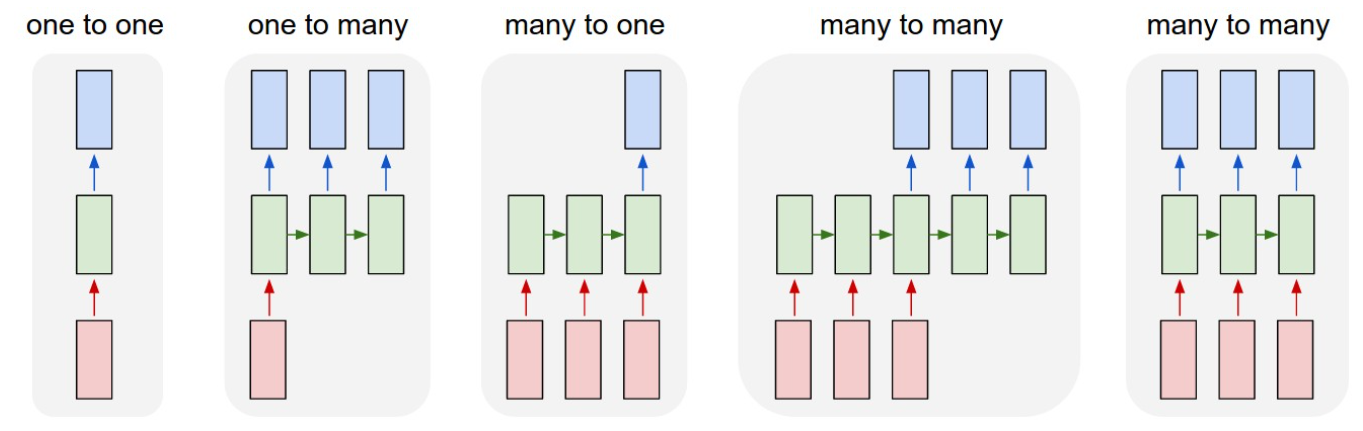
\includegraphics[width=15cm,height=15cm,keepaspectratio]{Figures/rnn.png}
    \caption{RNN problems}
    \label{rnn1}
\end{figure} \\ \newline \noindent Figure \ref{rnn2} shows the simplest version of an RNN, which can be easily derived from a simple feedforward architecture by adding a single loop:\begin{figure}[H]
    \centering
    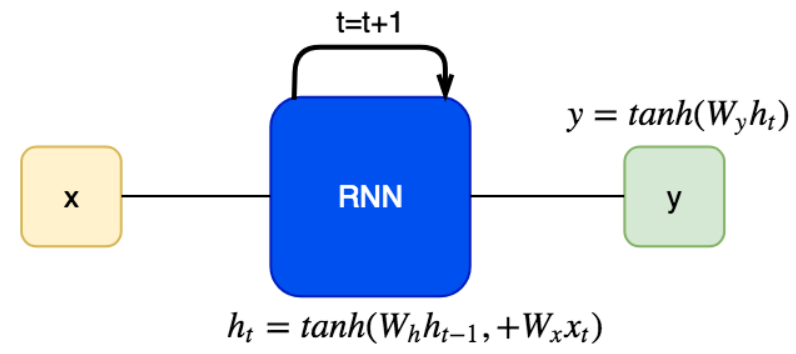
\includegraphics[width=15cm,height=15cm,keepaspectratio]{Figures/rnn2.png}
    \caption{Simplification of a RNN}
    \label{rnn2}
\end{figure} \\ \newline \noindent During training, the hidden state $h$ is iteratively updated based on the input value $x$ and the learned weights $W_h$  and $W_x$. The final output $y$  is estimated from the current state $h_t$  and the matrix $W_y$. Although RNN can assure short-term dependencies within the network, simple RNNs become unable to learn to connect information as the gap between past and present information grows \cite{lstm}. To overcome this limitation, in practical applications LSTM unit is adopted, that is a special RNNs architecture composed of multiple interacting layers.\begin{figure}[H]
    \centering
    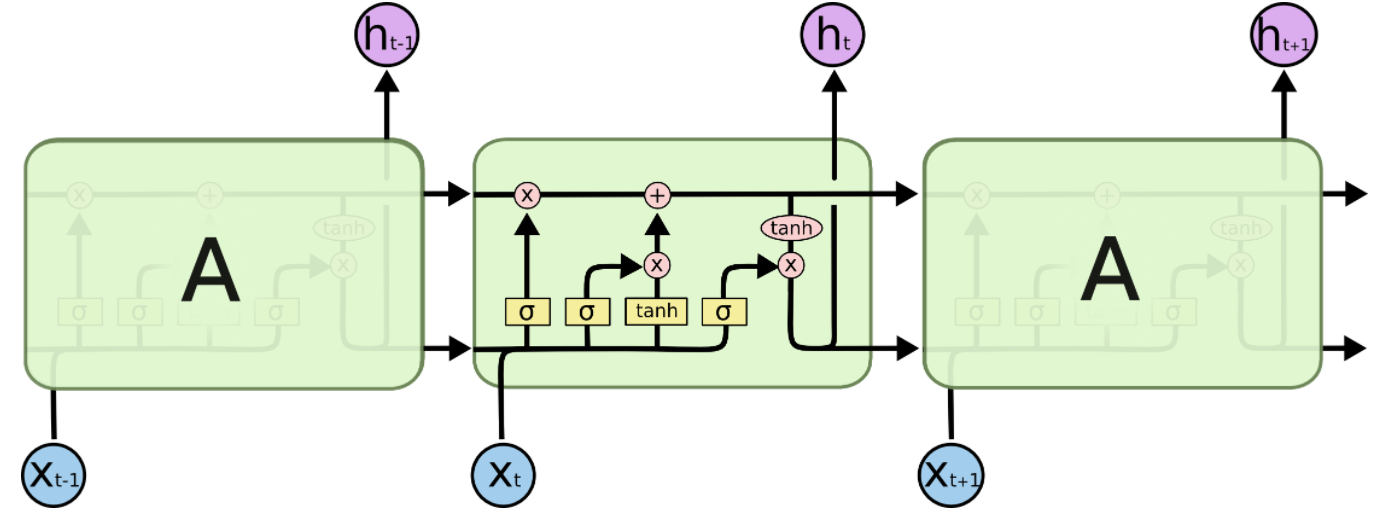
\includegraphics[width=15cm,height=15cm,keepaspectratio]{Figures/rnn3.png}
    \caption{LSTM network}
    \label{rnn2}
\end{figure} 

\subsection{Transformer Neural Networks (TNNs)}
RNNs are still quite used in several architectures and Natural Language Processing (NLP) tasks. However the Transformer Neural Network (TNN) has now started to outperform RNNs in several text/NLP benchmarks. A Transformer does not use any recurrence, it instead uses attention to focus on specific parts of a sentence \cite{deeplearning}. \\ \newline \noindent Both text classification and text generation tasks have been successfully tackled by transformers. Transformers seem to scale better than recurrent neural networks. They can have great results when using large architectures and large datasets, whereas RNNs seem not to benefit as much from using more parameters and training examples. State-of-the-art transformer models can have even billions of parameters and can benefit from training in terabytes of text data \cite{deeplearning}. \begin{figure}[H]
    \centering
    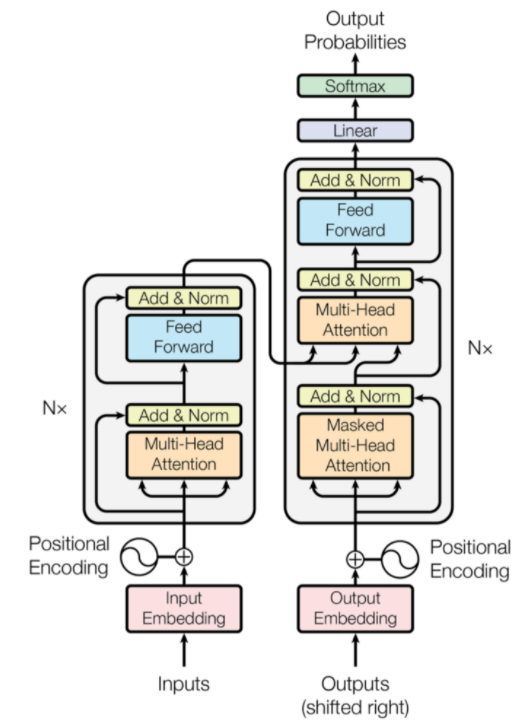
\includegraphics[width=10cm,height=10cm,keepaspectratio]{Figures/tnn.png}
    \caption{Model architecture for a transformer}
    \label{rnn2}
\end{figure} 

\subsection{Error metrics}
The two considered error calculations used in this experimentation are the Mean Absolute Error (MAE) and Root Mean Square Error (RMSE). They are defined by the following equations, \begin{align}
    MAE &= \frac{1}{N} \sum_{i=1}^N \lvert a_{i_{M}} - b_{i_{M}} \rvert \\
    RMSE &= \frac{1}{N} \sqrt{\sum_{i=1}^N \lvert a_{i_{M}} - b_{i_{M}} \rvert^2}
\end{align}\noindent In the context of BP estimation, $b_{i_{M}}$ and $a_{i_{M}}$ represent the true value and BP estimate respectively for the $M$th element of the time sequence.
\subsection{Literature Survey}
As a reference, the original literature survey matrix can be found on the Github repository \cite{LitSurvey}. Firstly, in Table \ref{litsurveytab}, a simplified literature survey has been detailed out for the best performing methods which do not employ machine learning methods. 
\begin{table}[H]
\begin{tabular}{|c|c|c|c|c|c|}
\hline
\textbf{Study} & \textbf{Source} & \textbf{No. Subjects} & \textbf{Age} & \textbf{Implementation} & \textbf{MAE SBP} \\ \hline
\cite{Ahmad2012} & ECG, PTT-CP & 10 & 24-63 & Numerical solution & \pm 5.93 \\
\cite{Chen2013} & ECG & 5 & N/A & Analytical solution &  9 \pm 5.6\\
\cite{Daimiwal2014} & PPG & 16 & 18-48 & Frequency analysis &  0.8 \pm  7\\
\cite{Chan2001} & ECG, PPG, PTT & N/A & N/A & Analytical solution &  7.49 \pm  8.8\\
\cite{Yamanaka2016} & PTT & 127 & N/A & Wavelet transforms &  \pm 7.63\\
\cite{Ding2016} & PTT, PPG & 27 & 21-29 & Analytical solution &  -0.37 \pm  5.21\\ \hline
\end{tabular}
\caption{Overview of performance of  the best non-invasive non-ML cuff-less methods for measuring BP}
\label{litsurveytab}
\end{table}

\begin{table}[H]
\begin{tabular}{|c|c|c|c|c|c|}
\hline
\textbf{Study} & \textbf{Source} & \textbf{No. Subjects} & \textbf{Age} & \textbf{Method} & \textbf{MAE SBP} \\ \hline
\cite{Yang2020} & ECG, PPG & 14 males & 17-43 & ANN & 7.99 \pm 10.34\\
\cite{Gao2016} & PPG & 65 & 22-65 & Wavelet, SVM & 5.1 \pm 4.3\\
\cite{Kachuee2015} & PPG & MIMIC II & Adults & Linear Reg., ANN, SVM &  13.84\pm  17.56\\
\cite{Simjanoska20182} & ECG & 51 & 16-83 & Complexity analysis + ML &  7.72 \pm  10.22\\ 
\cite{Wang2018} & PPG & 72 & N/A & ANN (MLP) & 4.02 \pm 2.79\\
\cite{Pradenas2020} & ECG, PPG & MIMIC II & Adults,  neonatal & ANN (150 neurons) & 5.76 \pm 6.39\\
\cite{Tanveer2018} & ECG, PPG & 39 & 20-100 & ANN-LSTM & 1.10\\
\cite{Chen2019} & PTT, ECG, PPG & MIMIC I & N/A & SVM, Lin Reg. & 3.27 \pm 5.52\\ 
\cite{Ripoll2019} & PTT & 250 & MIMIC I & ANN-RBM & 3.70\\\hline
\end{tabular}
\caption{Overview of performance of  the best non-invasive ML cuff-less methods for measuring BP}
\label{litsurveytab2}
\end{table} \\ \newline \noindent The Mean Absolute Error (MAE) of the Systolic BP (SBP) was used as the uniting accuracy measure in this paper, as it was the most readily available parameter in all of the aforementioned papers. \\ \newline \noindent It is important to note that other factors were considered in this literature survey. These factors were, \begin{itemize}
    \item Range of SBP and DBP values 
    \item Sampling frequency
    \item Denoising and detection techniques used
    \item Computational complexity
    \item Feasibility in a wearable context
\end{itemize}\noindent However, due to a lack of regular occurrences of these factors over all the papers, they were not included in the above two tables.\\ \newline \noindent The results show that the established non-ML methods do produce MAE values noticeably lower than the majority of the ML methods. However, a main factor to consider about these results is that machine learning based methods and neural networks are data driven. As shown in Table \ref{litsurveytab2}, there is a very limited number of subjects available for each study. If these studies had been extended to include more test patients, it is possible that these MAE SBP values were lower. An additional point is that another study \cite{Su2017} did a study into using a 4-layer LSTM architecture to estimate BP from ECG and PPG signals with 84 patients. This study resulted in an RMSE SBP of $3.9$ mmHg but no available MAE. Hence there is a lot of potential in ML methods when there is sufficient data available.


\newpage

\section{Implementation}
The scope of the project can be split into 4 sections, as detailed in the subsections below. The outcome of each task from each section forms a milestone. The full display of sections and tasks is provided in a Gantt chart \cite{Gantt} in the Appendix. The next 2 chapters will break down the respective sections of the chart.

\subsection{Project Research and Understanding}
 This section includes the following, as depicted in Figure \ref{gantt1}: \begin{enumerate}
    \item Exploration of literature on the heart and the underlying theory for blood pressure
    \item Investigation into existing experimentations conducted with wearable technologies for estimating blood pressure
    \item Research into signal denoising techniques and machine learning based methods for estimating BP
    \item Experimentation with the \textbf{Mind the Gap: The PhysioNet/Computing in Cardiology Challenge 2010} (later referred to as the PhysioNet 2010 database) \cite{challenge2010}
    \item Deciding on which methods to implement as a part of the project
\end{enumerate} \begin{figure}[H]
    \centering
    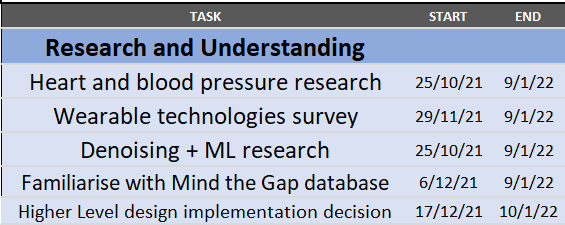
\includegraphics[width=10cm,height=10cm,keepaspectratio]{Figures/part1_gantt.png}
    \caption{Research and understanding matrix}
    \label{gantt1}
\end{figure} \noindent For the first three tasks, the milestone is to write Interim Report sections on that particular topic. These three sections have been explained in Chapters 2-4 of this report. The fourth task was more experimental, and the sole aim was for myself to become more comfortable with working with this database. The final task is the basis of the conclusion in Chapter 4. The work completed to date has been on schedule. Some of these tasks have had a larger time-span allocated to account for clashes with exams and coursework occurring at the beginning of the Spring Term.

\subsection{Implementation of chosen methods}
This section includes the following:
\begin{enumerate}
    \item The implementation of a Convolutional Neural Network (CNN) architecture    
    \item The implementation of a Recurrent Neural Network - Long Short Term Memory (RNN - LSTM) architecture
    \item The implementation of a Transformer Neural Network (TNN) architecture
    \item End-to-end testing of the three architectures
\end{enumerate}\begin{figure}[H]
    \centering
    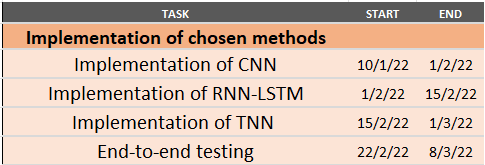
\includegraphics[width=10cm,height=10cm,keepaspectratio]{Figures/part2_gantt.png}
    \caption{Implementation of chosen methods matrix}
    \label{gantt2}
\end{figure} \noindent This section is the most crucial part of the project in terms of acquiring results. The BP estimation problem has been approached from 3 different directions: the CNN, the RNN-LSTM and the TNN architectures. The report section will include results of these unit tests, as well as a description of how the method functions and the process of programming the algorithm in Python. The main milestones for the first three points will be the comparison between the methods and unit testing. The last task in this section will be testing all methods from start to finish, with the aim to find any errors or bugs in the code. These tasks are currently set to take place during Spring term. However this may go beyond the set dates due to commitments from Spring Term coursework. This will be accounted for in the remaining 2 tasks to ensure the project progress is running on time.

\subsection{Performance Testing of methods}
This section includes the following:
\begin{enumerate}
    \item Testing the three methods with the PhysioNet 2010 database \cite{challenge2010}
    \item Testing the three methods with the MIMIC I database
    \item Testing the three methods with the MIMIC II database
    \item Applying any enhancements to the three methods based on results or new literature found
\end{enumerate}\begin{figure}[H]
    \centering
    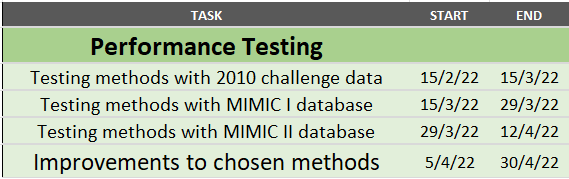
\includegraphics[width=10cm,height=10cm,keepaspectratio]{Figures/part3_gantt.png}
    \caption{Performance Testing matrix}
    \label{gantt3}
\end{figure} \noindent This section primarily consists of comparing the three methods on a variety of datasets. This section will also allow me to gather any information or data which may help to further optimise the methods used. The main milestones will be to gather this data and document the findings in the Final Report, along with potential reasons for the difference in performance. Extra time has been allocated to this stage due to exam commitments.
\newpage
\subsection{Assessment Preparation}
This section summarises the main deliverables which embody the Final Year Project, as well as my own modules which run at the same time. The tasks are as indicated in Figure \ref{gantt4}, \begin{enumerate}
    \item Literature survey presentation to supervisors
    \item Interim Report submission
    \item Accounting for commitments due to Spring Term coursework and Summer Term exams
    \item Writing up the Final Report
    \item Preparing for the final presentation
\end{enumerate} \begin{figure}[H]
    \centering
    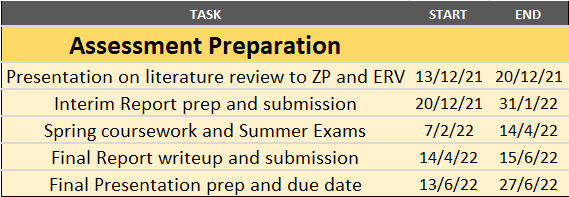
\includegraphics[width=10cm,height=10cm,keepaspectratio]{Figures/part4_gantt.png}
    \caption{Assessment Preparation matrix}
    \label{gantt4}
\end{figure} \noindent The first two tasks are now effectively completed. It was noted that the first task was beneficial in the writing of Chapters 2 to 4 in the Interim Report. Regarding the third task, in order to stay focused on  completion of the FYP, I will ensure to stay in regular weekly communication with my supervisor, and to ask any insightful questions where necessary. The final two tasks stem from successful completion of the FYP. 
\newpage

\section{Evaluation Metrics}
This section details how the success of each section will be measured, including backups in case a task for a particular section is not able to be completed.

\subsection{Project Research and Understanding}
The success of this section will be measured by the quality of the chapters of the Interim Report, in particular on the literature surveys. The report is the best factor to see how much has been understood during the Autumn and Spring Term. A primitive report draft was sent to my supervisor during this period to ensure information was concise, accurate and relevant. There is no definite backup plan for this section, except for implementing any changes based on the feedback for this report.

\subsection{Implementation of chosen methods}
Success is based on the output of the unit and end to end tests. If the methods all pass these tests by delivering similar results to those seen in the reviewed papers, then this is a total success. The main risk of this section will be the feasibility of implementing the solution in Python, i.e. whether it would take a deeper understanding of the mathematics or if certain capabilities are not possible in Python. If such a situation arises, the backup plan will be to switch to another programming language, such as MATLAB, or to implement another more suitable method, such as a wavelet-based method.

\subsection{Performance Testing of methods}
Success is based on the data acquired during the testing phase of the three potential methods. The Final Report is also an important indicator as it will detail the project findings. If balanced and suitable data, with regards to Ambulatory BP monitoring, is gathered for all of the potential methods under different use cases then this is seen as a total success. In addition, success is guaranteed if the report provides valid reasoning on the results. The main risk of this section is misunderstanding how the complexity can be correlated for the three different methods, leading to a misinterpretation of the results. The backup plan is to research more into the associated computational complexities when using these particular methods, to ensure a sound understanding of the principles. \\ \newline \noindent With regards to improving the existing methods further, success will be measured based on the figures from the updated methods, e.g. reduced complexities, increased accuracies. The main risk of this section is the possibility of not finding any improvements to be made. As these are already well researched methods internationally, the chances of finding improvements in the methods used are minimal. If a potential improvement isn’t found at all, then the backup plan is to organise a discussion meeting with the project supervisor.


\subsection{Assessment Preparation}
The success of this section will be based on several personal factors. Firstly, with regards to the project-related assessments, success will be measured based on how frequently I communicate with my FYP supervisors and how frequently I pose insightful questions that are beneficial to the development of my project. In addition, regular updates and additions to the Final Report as the Spring Term progressses will ensure that it is completed comfortably before the deadline of the $31^{st}$ of May 2022. Going forward, emails will be sent detailing major progress to my main supervisor contact (Dr Zaibaa Patel) and other supervisor (Professor Esther Rodriguez Villegas) every 2-3 weeks in the Spring term, with more frequent updates (1 week) targeted during the Summer term. Meetings will be held as and when required.

\newpage

\section{Databases for the project}
After having conducted a literature survey into the existing methods for estimating BP, I will now give an overview of what data will be used for this project.
\subsection{Literature survey data}
Referring back to the literature survey in Chapter 4, all of the studies used one of either Physionet's Multiparameter Intelligent Monitoring  in  Intensive  Care  (MIMIC) I  or MIMIC - II databases. \\ \newline \noindent The MIMIC Database includes data recorded from over 90 ICU patients. The data in each case include signals and periodic measurements obtained from a bedside monitor as well as clinical data obtained from the patient's medical record. The recordings vary in length; almost all of them are at least 20 hours, and many are 40 hours or more. In all, the database contains nearly 200 patient-days of real-time signals and accompanying data \cite{Moody1996}. The MIMIC-II database consists of 25,328 intensive care unit stays \cite{Saeed2011}.
\subsection{Data for this project}
The database which is used for current experimentation is the Physionet 2010 database \cite{challenge2010}. The samples were taken from ICU patient monitor recordings collected from the MIMIC II database. After this, the Physionet team made ten-minute records containing at least six simultaneous and continuous signals (digitized at 125 Hz each). The signals vary across each of the records. The signals primarily include ECG and PPG signals, but some do occasionally contain other signals, such as respiration. 300 monitor recordings were randomly chosen and a random ten-minute interval was chosen within each recording. In each ten-minute recording, the final thirty seconds of one of the signals, also chosen at random, was designated as the target signal and it was replaced by a flat line signal. The aim was to recreate this missing 30-second signal in each database recording. The modified records were assigned to one of the available data sets of 100 records each. It is noted that this assignment was also done at random: \begin{itemize}
    \item Set A is a training dataset of 100 records. The target signals were provided for the records in this set.
    \item  Set B was also a dataset of 100 records. However the target signals were not made available until the end of the competition.
    \item Set C is a set of 100 records, as was identical to Set B, in that the target signals were not made available.
\end{itemize} \\ \newline \noindent Once a greater understanding of this database has been developed, there will be future plans to implement data found in the MIMIC-I and MIMIC-II databases, in order to produce results more in line with those found in the previous literature survey. The most important consideration is that the dataset has minimal bias with regards to age, gender, etc.

\subsection{Software Implementation}
Python will be used as the sole programming language for this project. Python has a wide variety of easy to use and powerful libraries. These include scientific libraries such as \texttt{numpy} and \texttt{pandas} and machine learning libraries, including \texttt{tensorflow}, \texttt{keras} and \texttt{scikit-learn}. In addition the \texttt{wfdb-python} package will be installed, which is library of tools for reading, writing, and processing Waveform-Database (WFDB) signals and annotations. These are commonly found on the Physionet website. \\ \newline \noindent MATLAB was also considered as a potential programming language to use, due to it having a wide range of signal processing and machine learning add-on toolboxes. However Python has been shown to offer a wider set of choices in graphics packages and toolsets, such as through \texttt{matplotlib}, and it also produces more compact and readable code. \\ \newline \noindent Finally, a Github repository has been created for this project \cite{Github}. It will be constantly updated with Python code and supporting documentation throughout the Spring and Summer Terms and will function as an organised directory for all files used in this project.

\newpage

\section{Ethical, Legal and Safety Plan}

\subsection{Ethical considerations}
This section discusses the ethical implications of this project through the perspective of the Four Pillars of Medical Ethics: beneficence, non-maleficence, autonomy, and justice \cite{MedicalEthics}. 

\subsubsection{Beneficence}
Beneficence is the duty to do good. During the process of this project, it must be ensured that actions must be taken with the intent of helping patients. The purpose of future wearable technologies is to help people to detect early risk factors of heart-related pathologies. \\ \newline \noindent The issues that may arise would be due to the occurrence of false positives and negatives in the data, such as a normotensive result for a person who is actually hypertensive. Ideally, a blood pressure monitor which is cuffless should operate accurately over a range of blood pressure values after having been calibrated. However this has not been tested according to the established medical standards, such as AAMI and ESH. Measurements that are inaccurate will naturally cause a false sense of reassurance with the patients, unnecessary health care utilization, or improper administration of hypertension medications. An incorrect diagnosis also causes unnecessary psychological stress and the unnecessary reactions to the negative side effects of prescribed medication. For example, if there is a range of $\pm 5$ mmHg in error, this could lead to approximately twenty-seven million hypertensive and twenty-one million normotensive patients being classified incorrectly \cite{Bard2019}. This can only be minimised through robust tuning of the parameters in the neural networks used.

\subsubsection{Non-maleficence}
Non-maleficence is the duty to not harm. Through the recording of ECG and PPG data, it must be ensured that any actions must not be harmful to the patients. An instance where the product could harm patients would be if the models falsely classify a patient to be normotensive, whereas the patient indeed is hypertensive in real life. If test accuracy could be proven, it would be possible to see if a model is provably 100\% accurate, or otherwise justify to an Ethics Board that the risks would be worth the reward. However, with neural networks of this complexity, it is practically impossible to prove any estimate of test accuracy. 

\subsubsection{Autonomy}
Autonomy is the respect of patients' freedom of choice and consent. During the data acquisition process, it must be ensured that there are no actions taken that are non-consensual to the patients. Those concerned should also be informed about the benefits and risks of using a particular wearable technology product for BP measurement, such as the validation accuracy and inference time, allowing them to make an informed decision. \\ \newline \noindent Another general issue of using deep neural networks is that it is very difficult to explain how models obtain their results. It is impossible to explain what features an individual or end-to-end model detects and what any of their weights correspond to. This can be an issue if the user wants an explanation as to why they have been classified wrongly as hypertensive or hypotensive, as they should have the right to know.

\subsubsection{Justice}
Justice is the principle of fairness towards all patients and the idea of treating all people equally and equitably. The product must ensure it does not discriminate between patients and medical staff on any basis. An obvious concern is whether the dataset used to train the models are balanced in representing both gender and ethnicity. Although the dataset was created taking such biases into account, it is difficult to overcome subconscious biases and availability of a balanced dataset. This is important as it ensures that future products in wearable technologies have both a sustainable customer base but is also sustainable in today's social ecosystem, as it is actively standing against racism.

\subsection{Legal considerations}
Legally this project poses no risk. The Python programming language and its required libraries are Open Source, including the version which I intend to use (3.10). Python has a license agreement under the Python Software Foundation (PSF). Hence it is a tool that can be legally used freely for the purposes of this project. \cite{Python}. In addition, the ECG and PPG data is provided by a website called Physionet. PhysioNet is a data repository of medical signals which are free to use. The repository is managed by the MIT Laboratory for Computational Physiology \cite{Goldberger2000} \cite{Physionet}. As this code will be published online, the produced code could be plagiarised in the future. However, I myself will bear no responsibility in the distribution of my code to others.

\subsection{Safety considerations}
With regards to this project, there are no safety issues to consider, as all experimentation will be conducted online at home. It is critical that necessary measures are taken such that strains or injuries from desk work are prevented. This can easily be done by following NHS guidelines. \\ \newline \noindent 
As highlighted in Chapter 3, there are a few points to consider if this work becomes implemented in a future wearable technology product. Firstly, it is important to remember these are only simulations. Training a machine learning model on Python will not accurately reflect the behavior in real life. Secondly, any results discussed in this report will not be officially recognised by the AAMI or ESH protocols. This is something that future active projects will need to consider, in order to have substantial results.

\newpage

\section{Current experimentation}
The aim of this experimentation is to evaluate six implementations which were used in the Physionet 2010 database. These are detailed in Table \ref{tab_experimentation}, \begin{table}[H]
    \centering
\begin{tabular}{|c|c|c|}
\hline
\textbf{Name} & \textbf{University} & \textbf{Method used} \\ \hline
András Hartmann & Semmelweis University, Hungary & Adaptive Filtering \\
Mohamed Mneimneh & Sahar Elturk Marquette University, USA & Kalman Filtering \\
Ikaro Silva & MIT, USA & Kalman and Adaptive Filtering \\
Adam Sullivan et al. & University of Tennessee, Knoxville, USA & Artificial Neural Networks \\
Rui Rodrigues & Universidade Nova de Lisboa, Portugal & Neural Networks \\
Luiz Silva et al. & University of São Paulo, Brazil & Recurrent Neural Networks \\
 \hline
\end{tabular}
\caption{Overview of most popular methods used in the 2010 Challenge \cite{challenge2010}}
\label{tab_experimentation}
\end{table} \\ \newline \noindent It is noted that the first three methods adopt signal processing and filtering techniques \cite{hartmann} \cite{mneimneh} \cite{iSilva} and the other three methods implement machine learning based methods \cite{lSilva}  \cite{rodrigues} \cite{sullivan}. \\ \newline \noindent For the benefit of this project, I wanted to recreate their implementations to justify the choice of using machine learning based methods to estimate BP from ECG and PPG signals. The metric to compare all six implementations was the aggregated scores of the models on Set C of the previously mentioned PhysioNet 2010 database \cite{challenge2010} $C_1$ is a parameter between 0 and 100 which scores the overall accuracy of the reconstructed signal by the methods. $C_2$ is a similar parameter which instead measures the correlation between the original and reconstructed signals. Hence the final performance results are shown in Figure \ref{lol}, \begin{figure}[H]
    \centering
    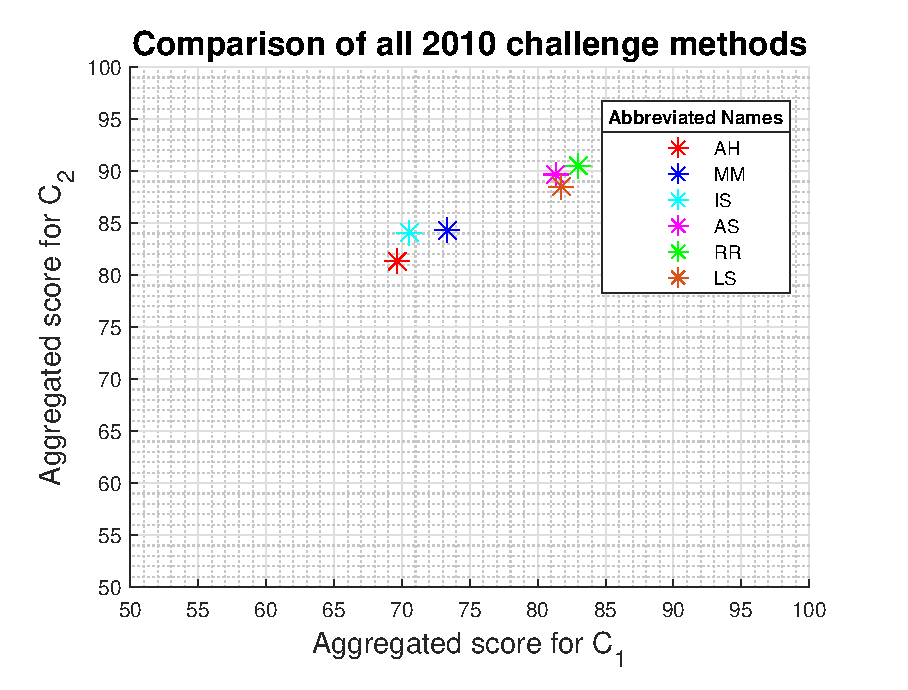
\includegraphics[width=14cm,height=14cm,keepaspectratio]{Figures/challenge2010.eps}
    \caption{Performance of all implementations used in the 2010 CIC challenge}
    \label{lol}
\end{figure} \\ \newline \noindent As the results in Figure \ref{lol} show, the machine learning methods appear to reconstruct the ECG signals much more effectively than the signal processing based methods. This is a chapter that will require more depth but for now, it shows promising signs that a machine learning method will be more effective in estimating blood pressure from at least ECG signals. An important point to note is that there were no Convolutional Neural Network (CNN) or Transformer Neural Network (TNN) methods available to implement on this dataset. In order to be in line with the arguments made in this report, a viable step would be to see the performance of a CNN on the Physionet 2010 database.



\newpage

\section{Conclusion}
In Chapter 1, the project deliverables were highlighted and a motivation was provided to complement the background information. In Chapter 2, detailed background information was given on a variety of topics. Firstly, on hypertension, a significant disease associated with the heart. After this, the principles of blood pressure measurements were discussed, as well as the fundamentals of ECG and PPG signals. Finally, the underlying theory for PTT, PAT and PWV were discussed. In Chapter 3, an overview of the existing wearable implementations for estimating blood pressure were discussed, with smart watches being viewed as the most viable option due to the prevalence of accurate data. In Chapter 4, a literature survey was taken to assess the potential methods to estimate blood pressure from ECG and PPG signals. As a result, machine learning methods were favoured over adaptive filtering, wavelet-based and numerical methods. The implementation and evaluation plans were given in Chapters 5 and 6 respectively. After this, more information on the data used and the Ethical, Legal and Safety considerations were discussed. \\ \newline \noindent The immediate future tasks are to implement each of the viable methods in Chapter 4 in Python and to begin to record results for the necessary chapters in the Final Report. In addition, a study will be taken into the existing denoising techniques used on the ECG and PPG waveforms, in order to assess what is suitable for this project. Finally, more empirical analysis is needed to assess the effects of complexity on the implementations. One potential factor which can be used to measure the effects of complexity on neural networks is the inference time.
\newpage

\section{Appendix}
\subsection{Miscellaneous Points}
\begin{itemize}
    \item The Advancement of Medical Instrumentation (AAMI) standard requires a mean BP difference of $\le 5$ mmHg with a standard deviation of $\le 8$ mmHg against auscultatory reference measurement
    \item Significant variation in BP measurements($\gt 12$ mmHg systolic or $\gt 8$ mmHg diastolic) from the validated reference device is an exclusion criterion in the AAMI protocol \cite{Bard2019}
    \item The European Society of Hypertension (ESH) protocol requires that the majority of subjects have investigational BP readings within $\le 5$ mmHg of the reference measurement.
\end{itemize}

\subsection{Gantt Chart}
\begin{figure}[H]
    \centering
    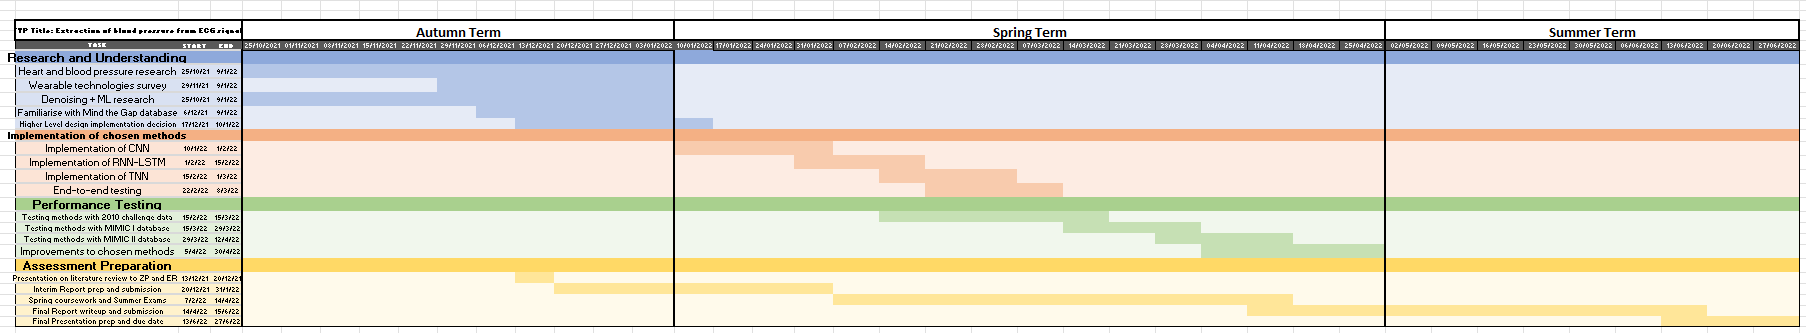
\includegraphics[width=18cm,height=18cm,keepaspectratio]{Figures/gantt.png}
    \caption{Gantt Chart}
    \label{gantt}
\end{figure}


\newpage
\bibliographystyle{ieeetr}
\bibliography{references}
\newpage
\end{document}